\section{Systematisk Test af Program}
\label{sec:systematisk_test_af_program}

\subsection{Test Driven Development}
\label{sub:test_driven_development}

\kanote{fokus på 'målet', overvej sætningskonstruktion. definér `nem at kalde'.}

For at sikre at programmet er let at teste, er kernefunktionerne i programmet udviklet jævnfør softwareudviklingsprocessen \enquote{Test Driven Development}. I Test Driven Development (TDD) skrives unit tests af en metode, før selve implementeringen af funktionen. Denne udviklingsprocess sikrer, at nye funktionaliteter ikke ødelægger de forud eksisterende \cite{martin2006agile}. Programmøren tvinges også til at tænke på, hvordan metoden bruges ved kald. Det sikres hermed, at metoden er overskueligt konstrueret, således at den kan kaldes uden unødigt besvær. Et andet aspekt af TDD, er at testkoden tjener dokumentation af den testede metodes funktionalitet.

\subsection{Unit Testing i Microsoft Visual Studio}
\label{sub:unit_testing_i_microsoft_visual_studio}

Microsofts unit test framework for managed code er anvendt til unit testing. Frameworket kan teste \enquote{managed code}, som c\# falder ind under. Når tests er skrevet, kan Test Explorer i Visual Studio køre testene. Når testene er færdige, vil resultaterne blive præsenteret som failed tests, passed tests, not run tests og skipped tests \cite{msdn_unittest}.

Før der skrives unit tests, skal der oprettes et unit test projekt. Herefter kan der tilføjes klasser annoteret med \enquote{[TestClass]}. Inde i disse klasser, tilføjer man de metoder, annoteret med \enquote{[TestMethod]}, som skal køres. Et eksempel på en test metode, kan se i \cref{lst:test_notfound}.
Alle tests til systemet kan findes på CD'en der afleveres som bilag.

\begin{lstlisting}[label=lst:test_notfound, caption={Eksempel på testfunktion}]
  [TestMethod]
  public void ShouldThrowWhenNotFound()
  {
      var space = new WaterSpace(404404, 4.3, 5.4);
      try
      {
          var test = BoatDetector.BoatAt(space);
      }
      catch (KeyNotFoundException _)
      {
          return;
      }
      Assert.Fail("No exception was thrown.");
  }
\end{lstlisting}



\begin{figure}
  \centering
  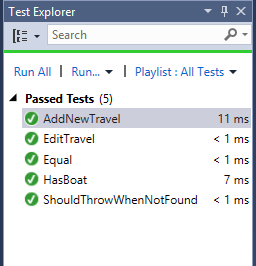
\includegraphics{test_explorer.png}
  \caption{Resultat af tests i Test Explorer i Visual Studio 2013}
  \label{fig:test_explorer}
\end{figure}
